% Specify the type of document
\documentclass[12pt]{article}

% Load a number of useful packages
\usepackage{graphicx}
\usepackage{amsmath,amssymb,amsfonts,amsthm}
 \usepackage[margin=1.0in]{geometry}
\usepackage[colorlinks=true]{hyperref}
\usepackage{cite}
\usepackage[caption=false,font=footnotesize]{subfig}
\usepackage{wrapfig}

% Two more packages that make it easy to show MATLAB code
\usepackage[T1]{fontenc}
\usepackage[framed,numbered]{matlab-prettifier}
\lstset{
	style = Matlab-editor,
	basicstyle=\mlttfamily\small,
}


% Say where pictures (if any) will be placed
\graphicspath{{./pictures/}}

% Define title, author, and date
\title{AE353: Design Problem 04}
\author{T. Bretl \textbf{(this is my name, not your name!)}}
\date{April 11, 2019}

% Start of document
\begin{document}

% Put the title, author, and date at top of first page
\maketitle


\section{Goal}

\begin{wrapfigure}[15]{r}{0.45\textwidth}
\vspace{-6em}%
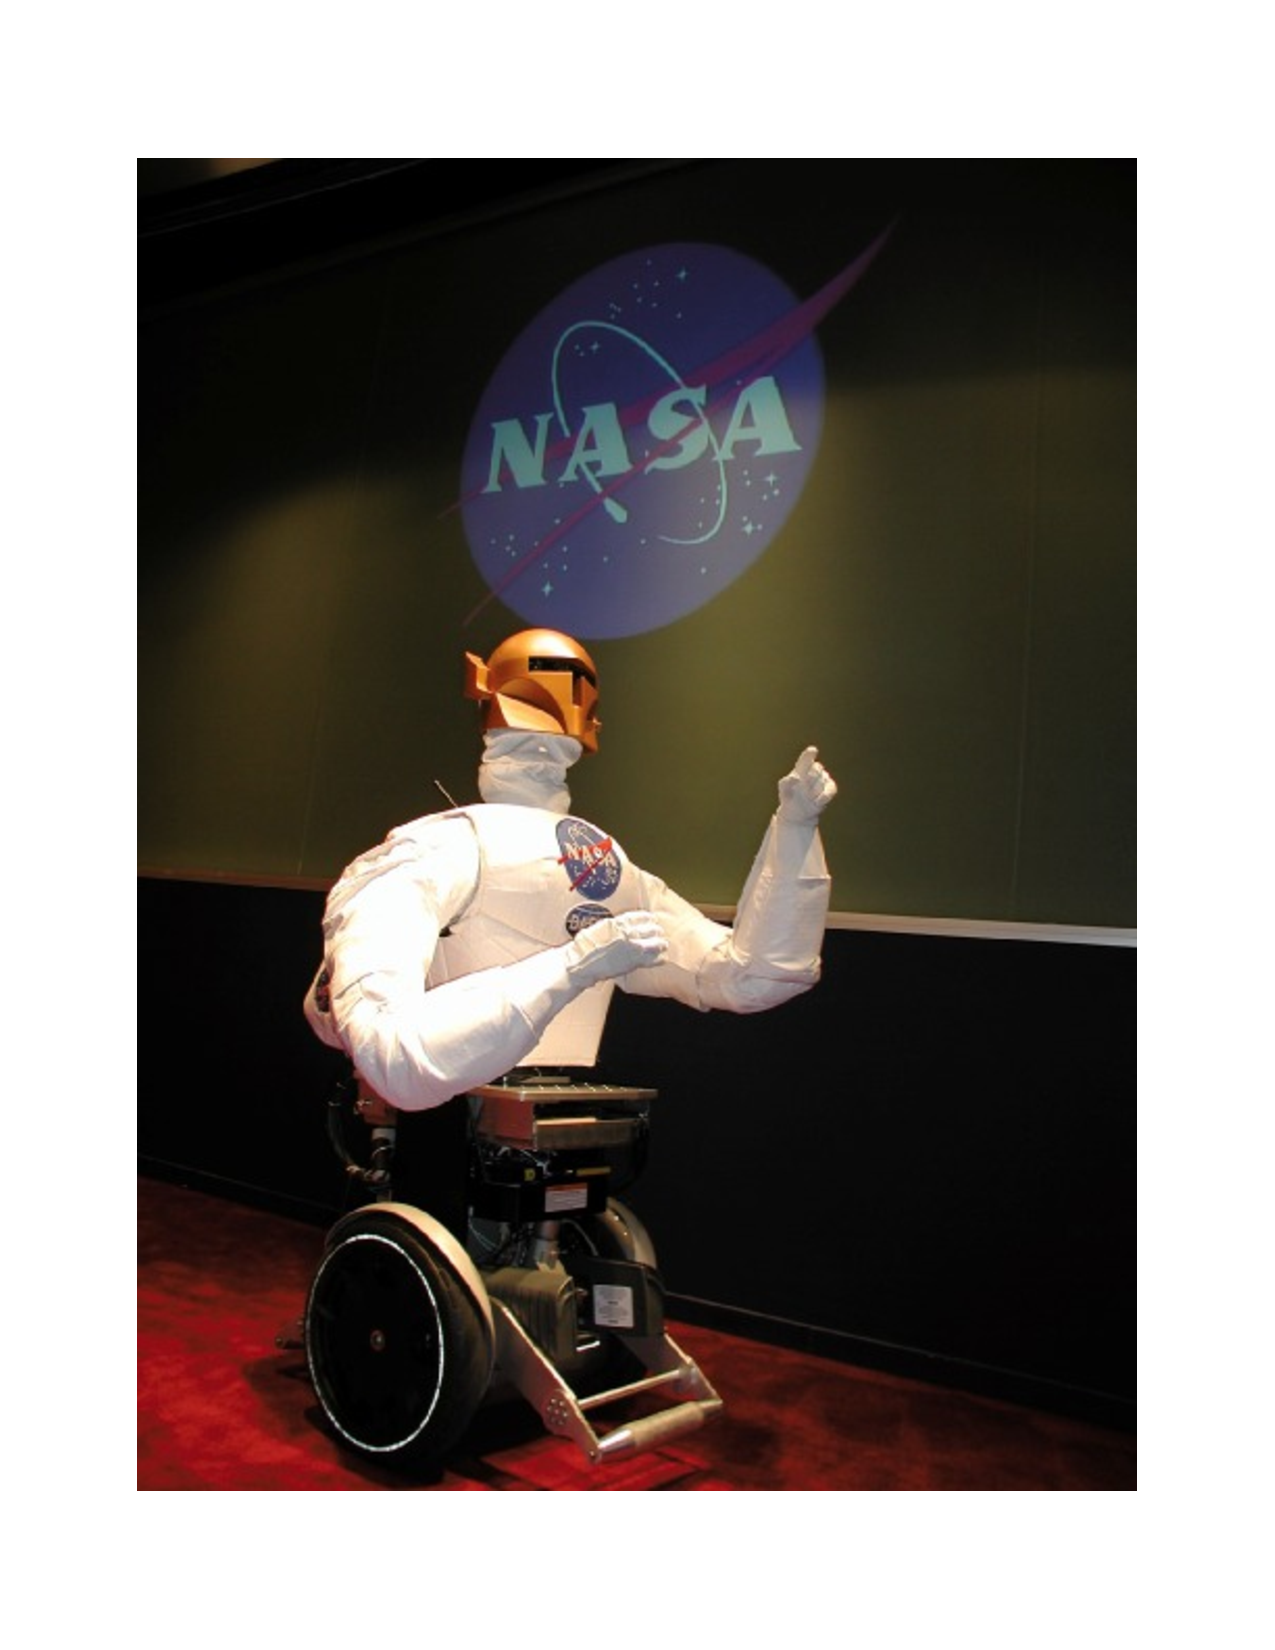
\includegraphics[width=0.4\textwidth]{robonaut}
\vspace{-3em}
\caption{The NASA robonaut on top of a segway robotic mobility platform (\url{http://spaceflight.nasa.gov/gallery/images/station/eva/html/jsc2005e11678.html}). \label{figRobonaut}}
\end{wrapfigure}

The code provided in \lstinline!DesignProblem04! simulates a two-wheeled robot that is similar to the segway robotic mobility platform\footnote{See also \url{http://www.segwayrobotics.com}.}, which has been considered for use with the NASA robonaut (Figure \ref{figRobonaut}). Actuators allow you to specify the torque applied to each wheel. Sensors allow you to measure the angular velocity of each wheel. Sensors also allow you to measure the turning radius of a road along which the robot can drive, as well as the error in lateral position and the error in heading relative to this road. The goal is to make the robot race along this road---without crashing---as fast as possible.

\section{Model}

\subsection{Robot dynamics}
\label{secRobot}

The motion of the robot is governed by ordinary differential equations with the form
\begin{equation}
\label{eqEOM}
\begin{bmatrix} \ddot{\phi} \\ \dot{v} \\ \dot{w} \end{bmatrix} = f(\phi,\dot{\phi},v,w,\tau_{R},\tau_{L})
\end{equation}
where $\phi$ is the pitch angle of the chassis, $\dot{\phi}$ is the pitch angular velocity, $v$ is the forward speed, $w$ is the turning rate, and $\tau_{R}$ and $\tau_{L}$ are the torques applied by the chassis to the right and left wheel, respectively \cite{Mak2015,Tobias2014}. The function $f$ in \eqref{eqEOM} depends on a number of parameters (e.g., lengths, masses, moments of inertia). You can access a symbolic description of this function either within your controller code (\lstinline|Controller.m|) as \lstinline|parameters.symEOM.f|, or in a separate piece of code that you write for the purpose of control design. In particular, the first time you run \lstinline|DesignProblem04|, it will create a file that you can load to access the equations of motion. Here is an example:
\begin{quote}
\begin{lstlisting}
% Load the equations of motion.
load('DesignProblem04_EOMs.mat');
% Parse the equations of motion.
f = symEOM.f;
% Define symbolic variables that appear in the equations of motion.
syms phi phidot v w tauR tauL real
% Proceed to linearize or do whatever else you like...
%     (see: help sym/jacobian, help sym/diff, help sym/subs, etc.)
\end{lstlisting}
\end{quote}
The simulator integrates three more equations of motion that relate the forward speed $v$ and turning rate $w$ to the position $(x,y)$ and orientation $\theta$ of the robot:
\begin{align*}
\dot{x} &= v\cos\theta \\
\dot{y} &= v\sin\theta \\
\dot{\theta} &= w.
\end{align*}
However, for the purpose of control design to follow a road, it is probably more useful to keep track of the position and orientation {\em relative to the road} and not with respect to an absolute reference frame. In particular, suppose you know the radius of curvature $r_\text{road}$ of the road along which the robot is currently moving (where $r_\text{road}>0$ means turning left, $r_\text{road}<0$ means turning right, $r_\text{road}=0$ means turning in place, and $r_\text{road}=\infty$ means going straight). Then, given a speed $v_\text{road}$ at which you would like to travel along the road, the turning rate $w_\text{road}$ necessary to follow its centerline can be computed as
\begin{equation}
\label{eqCurvature}
w_\text{road} = \frac{v_\text{road}}{r_\text{road}}.
\end{equation}
Now, define $e_\text{lateral}$ as the perpendicular distance from the centerline of the road to the position $(x,y)$ of the robot (where $e_\text{lateral}>0$ means being too far to the right and $e_\text{lateral}<0$ means being too far to the left), and define $e_\text{heading}$ as the difference between the orientation $\theta$ of the robot and the direction of the road. It is possible to show that
\begin{equation}
\label{eqErrorEOM}
\begin{aligned}
\dot{e}_\text{lateral} &= -v\sin\left(e_\text{heading}\right) \\
\dot{e}_\text{heading} &= w-\left(\frac{v\cos\left(e_\text{heading}\right)}{v_\text{road}+w_\text{road}e_\text{lateral}}\right)w_\text{road}.
\end{aligned}
\end{equation}
A complete set of nonlinear equations of motion for the purpose of control design can be obtained from \eqref{eqEOM} and \eqref{eqErrorEOM}---with states $e_\text{lateral}, e_\text{heading}, \phi, \dot{\phi}, v, w$ and inputs $\tau_{R},\tau_{L}$---augmented as usual with a differential equation that describes $d(\phi)/dt$.

Sensors allow you to measure the lateral error ($e_\text{lateral}$), the heading error ($e_\text{heading}$), and the radius of curvature ($r_\text{road}$) at the point on the road that is closest to the robot at any given time. Sensors also allow you to measure the angular velocity of both the right wheel ($w_{R}$) and the left wheel ($w_{L}$), where positive means rolling forward and negative means rolling backward. You may assume that both wheels roll without slipping. Both the radius $r$ of each wheel and the distance $b$ between the wheels are available in \lstinline|parameters|. Given this information, you should be able to express both $w_{R}$ and $w_{L}$ in terms of the forward speed $v$ and turning rate $w$---you'll need to do so in order to model your sensors, so speak up right away if you have questions.\footnote{The dynamics reference pages from TAM212 on rigid bodies (\url{http://dynref.engr.illinois.edu/rkg.html}) and on rolling motion (\url{http://dynref.engr.illinois.edu/rko.html}) may be helpful.}

\subsection{Road}

The road is defined by its centerline, which has piecewise-constant curvature. You can create a new, random road (saved by default to the file \lstinline|'road.mat'|) by calling the function \lstinline|MakeRoad|. This road will be a sequence of circular arcs, placed one after another. The array \lstinline|road.s| stores the length of each arc. The array \lstinline|road.w| stores the curvature of each arc. You need not worry about these data structures (unless you want to hand-design your own roads, for the purpose of testing)---your controller will not have access to them. Instead, as described in Section \ref{secRobot}, your controller will know the lateral error ($e_\text{lateral}$), the heading error ($e_\text{heading}$), and the radius of curvature ($r_\text{road}$) at the point on the road that is closest to the robot at any given time. This information is available in \lstinline|sensors|, as usual.

\subsection{Variables}

This section provides extra information about how variables are named in \lstinline|DesignProblem04|, to avoid confusion. The function $f$ in \eqref{eqEOM} is provided in MATLAB as \lstinline|parameters.symEOM.f|. The inputs to this function are:
\begin{itemize}
\item $\phi$, the chassis angle, called \lstinline|phi| in MATLAB
\item $\dot{\phi}$, the time derivative of the chassis angle, called \lstinline|phidot| in MATLAB
\item $v$, the forward speed, called \lstinline|v| in MATLAB
\item $w$, the turning rate, called \lstinline|w| in MATLAB
\item $\tau_{R}$ and $\tau_{L}$, the right and left motor torques, called \lstinline|tauR| and \lstinline|tauL| in MATLAB
\end{itemize}
You can initialize these variables as follows:
\begin{quote}
\begin{lstlisting}
syms phi phidot v w tauR tauL real
\end{lstlisting}
\end{quote}
The extra two equations of motion in \eqref{eqErrorEOM} are not provided in MATLAB. You will have to define them. The extra variables in these equations are:
\begin{itemize}
\item $e_\text{lateral}$, the lateral error in following the road, called \lstinline|e_lateral| in MATLAB
\item $e_\text{heading}$, the heading error in following the road, called \lstinline|e_heading| in MATLAB
\item $v_\text{road}$ and $w_\text{road}$, the forward speed and turning rate of a trajectory that would follow the road centerline, called \lstinline|v_road| and \lstinline|w_road| in MATLAB---remember that $w_\text{road}$ can be computed as in \eqref{eqCurvature}, given a choice of $v_\text{road}$ and given the radius of curvature $r_\text{road}$, called \lstinline|r_road| in MATLAB
\end{itemize}
You can initialize these extra variables as follows:
\begin{quote}
\begin{lstlisting}
syms e_lateral e_heading v_road w_road real
\end{lstlisting}
\end{quote}
Note that $v_\text{road}$ and $w_\text{road}$ are not states---they are parameters on which your model might depend. Also note that you have choice over the names you use to describe variables in the equations of motion \eqref{eqErrorEOM}, since you'll be defining these equations yourself (they are not given to you in \lstinline|DesignProblem04|). However, the names listed above are recommended.


\section{Tasks}


\subsection{Analysis}
\label{secAnalysis}


The focus of your analysis this time will be on identifying, diagnosing, and eliminating failure modes. ``Failure'' for the robot is a crash---either running off the road or dropping the chassis. There are many reasons why a particular control design might lead to failure, on certain roads or in certain situations. Your job as a control engineer is to uncover and address these sources of failure. At minimum, you should consider at least three different control designs, and for each design, you should do the following:
\begin{itemize}
\item Identify at least one road that causes failure.

(Remember---a failed experiment is a blessing! Then you can address the source of the failure. There are always failure modes, and sometimes these are very hard to find.)

\item Say why the failure occurred, providing evidence to support your argument.

(Was there a large error in the state estimate? Did your control design exceed the maximum torque in each wheel? Is there a limit on how tight a turn your control design can handle, and can you quantify this limit? Thinking of the road as a source of disturbance in the closed-loop system, do failures have something to do with characteristics of the frequency response? These are examples of questions you might ask when thinking about causes of failure.)

\item Suggest a change to the control design that would eliminate the failure, and verify in simulation that it does.

(Sometimes, it is impossible to eliminate a failure mode. If you believe that this is the case, and that you have reached a fundamental limit in the performance of the robot, provide evidence for this claim.)

\end{itemize}
Remember that you have a lot of practice in doing rigorous data collection, analysis, and visualization---this was the focus of the third design problem, and can help a lot in identifying and diagnosing failure modes. Also remember that (in general) your observer has to be working well in order for your controller to work well. So, one good place to look for causes of failure is the error in your state estimate.

\subsection{Presentation}

The focus of your presentation this time will be on citations. For example, suppose you want to quote a result that appears in the first edition of the textbook ``Feedback Systems: An Introduction for Scientists and Engineers,'' which was written by Karl Astr{\"o}m and Richard Murray. To do this in \LaTeX\, you would do the following:
\begin{itemize}
\item Create a file called \verb|references.bib| and add it, for example, to the list of files in your overleaf project (you'll note that a ``bib file'' like this one is being used to generate this document---you can use it as a template).
\item Add the following text to this file:
\begin{quote}
\mlttfamily\scriptsize
\begin{verbatim}
@book{Astrom2010,
  title={Feedback Systems: An Introduction for Scientists and Engineers},
  author={K. J. Astr{\"o}m and R. M. Murray},
  isbn={9781400828739},
  edition={First},
  url={http://www.cds.caltech.edu/~murray/amwiki/index.php/First_Edition},
  year={2010},
  publisher={Princeton University Press}
}
\end{verbatim}
\end{quote}
\item Add the following text in your main document, where you want to cite the book:
\begin{quote}
\mlttfamily\scriptsize
\verb|\cite{Astrom2010}|
\end{quote}
For example, you may want to say something like the following:
\begin{quote}
\mlttfamily\scriptsize
\begin{verbatim}
Robustness of the closed-loop system to time delay was verified
by analysis of the Nyquist plot \cite{Astrom2010}.
\end{verbatim}
\end{quote}
\item Add the following text to your main document, just before the call to \verb|\end{document}|:
\begin{quote}
\mlttfamily\scriptsize
\begin{verbatim}
% Display list of references in IEEE format.
\bibliographystyle{IEEEtran}
\bibliography{IEEEabrv,references}
\end{verbatim}
\end{quote}
\item Make sure the following line appears near the top of your main document (it makes citations look nicer):
\begin{quote}
\mlttfamily\scriptsize
\begin{verbatim}
\usepackage{cite}
\end{verbatim}
\end{quote}
\end{itemize}
When you compile your document, all calls to \verb|\cite{...}| will be replaced by numbered references \verb|[...]|, which correspond to items in the list that will appear at the end of your document. For example, here is a citation to Astr{\"o}m and Murray, exactly as described\cite{Astrom2010}. There is a lot more information online about how to create, manage, and use bibliographies with latex documents\footnote{For example: \url{https://www.overleaf.com/help/97-how-to-include-a-bibliography-using-bibtex}.}. Do not hesitate to ask for help. At minimum, you should include at least one citation (other than to Astr{\"o}m and Murray) in your report.

\subsection{Process}

Your report will include the following four parts:
\begin{itemize}

\item Define one requirement and one verification.

\item Derive a model (i.e., linearize the equations of motion and express your result in state-space form).

\item Design a controller and an observer (remembering to check, first, that your linearized model is both controllable and observable).

\item Implement and test your control design in simulation. Follow the instructions you wrote to verify that your requirement has been satisfied. Identify, diagnose, and eliminate at least one source of failure in at least three different designs (see Section \ref{secAnalysis}).

\end{itemize}
As usual, you are encouraged to go beyond these requirements.

\section{Contest}

There will be an opportunity to race against your friends in a friendly competition on the last day of class (Wednesday, May 1). The code that will be used to run this race is \lstinline|DesignProblem04Race.m|. The key difference between this and \lstinline|DesignProblem04.m| is that, rather than requiring you to specify a single controller, the race code requires you to specify the name of a folder in which you can put any number of controllers. A robot will be created for each controller in the folder---all will race at the same time. To test your controller in race conditions, do the following:
\begin{itemize}
\item Put the controllers you want to test in the folder \lstinline|DesignProblem04/racers|.
\item Open MATLAB and make \lstinline|DesignProblem04| your working directory.
\item Seed the random number generator:
\begin{quote}
\lstinline|rng('shuffle');|
\end{quote}
\item Make a road:
\begin{quote}
\lstinline|MakeRoad('road.mat');|
\end{quote}
\item Run the simulation (there are some optional parameters to play with, if you like):
\begin{quote}
\lstinline|DesignProblem04Race('racers','road.mat');|
\end{quote}
\item If desired, show the results:
\begin{quote}
\lstinline|ShowResults('racers/results.mat');|
\end{quote}
\end{itemize}
There are three small but important differences in your controllers for the race:
\begin{itemize}
\item The race code enforces a bound on computation time. If your ``runControlSystem'' function takes more than 0.02 seconds on my laptop to execute on five separate occasions, your controller will be turned off (disqualified). Note that my computer will likely run your code at least as fast as your computer, but please err on the safe side.
\item The race code enforces a strict prohibition on printing anything to the command window (e.g., the result of forgetting to put a semicolon at the end of a line). If either your ``initControlSystem'' function or ``runControlSystem'' function prints anything to the command window, your controller will be turned off (disqualified). Please check carefully that it does not!
\item The race code allows each controller to---if desired---specify its own value of ``iDelay'' (the number of time steps that sensor data will be delayed). Look at the example \lstinline|racers/netid_controller.m| to see how this is done. If you make no change to your controller code, that's fine---the default is \lstinline|iDelay = 0|. If you choose to change your controller code to specify a non-zero delay, then your total time will be reduced by a number of seconds equal to \lstinline|2 * iDelay| (so, if \lstinline|iDelay = 10|, then your time will start at $-20$ seconds).
\end{itemize}
To compete in the race, you must submit your code by the deadline (see below). All submitted controllers will race in a qualifying round. The top 9 finishers will advance to the semifinals (in 3 groups of 3). The top finishers in each semifinal round will advance to the finals (in 1 group of 3). The qualifying round will be done before class---the results will be revealed at the start of class (on May 1). The semifinal and final round will be done in class. The winner of the final round will receive a prize. You {\bf must} be present in class to compete in the semifinal/final round and to receive a prize.

Note that this race is just for fun. Although you are required to submit your code to the race, the results have no impact at all on the assessment of your fourth design report.

\section{Deliverables}


\subsection{First draft}

You must submit one thing by 11:59PM on Thursday, April 18, 2019:
\begin{itemize}
\item A PDF document that was generated using \LaTeX\ and that includes, at minimum, a draft of your requirement and verification and of your state-space model.
\end{itemize}
Please submit this draft report at the following URL:
\begin{quote}
\url{https://forms.illinois.edu/sec/4918175}
\end{quote}
You may submit as many times as you want---only the latest submission will be recorded. So please, submit early and often.

\subsection{Second draft}

You must submit one thing by 11:59PM on Thursday, April 25, 2019:
\begin{itemize}
\item A PDF document that was generated using \LaTeX\ and that includes, at minimum, a draft of your requirement and verification, of your state-space model, of your control design and analysis, and of your results in simulation.
\end{itemize}
Please submit this draft report at the following URL:
\begin{quote}
\url{https://forms.illinois.edu/sec/6075281}
\end{quote}
You may submit as many times as you want---only the latest submission will be recorded. So please, submit early and often.

\subsection{Final report}

You must submit four things by 11:59PM on Monday, April 29, 2019:
\begin{itemize}

\item Code --- Controller and Test. The controller code will be written in MATLAB, using the template \lstinline!Controller.m!. The test code will be written in MATLAB, using the template \lstinline|Test.m|. If \lstinline|Test.m| is executed by one of your peers in a folder with your controller code \lstinline!Controller.m!, the simulation code \lstinline!DesignProblem04.m!, the road-making code \lstinline|MakeRoad.m| (so, {\em not} a \lstinline|road.mat| file---your test code will have to use \lstinline|MakeRoad.m| to create one), and a file with the equations of motion \lstinline|DesignProblem04_EOMs.mat|, it will produce results that verify your requirement has been satisfied. {\em The controller code that you submit will also be used in the race!}

\item Report --- PDF and Source Files. This report will be written in \LaTeX. You will submit both a PDF document and the \LaTeX\ source files that you used to produce this document. The PDF document must be four pages. The source files must be in a ZIP folder and must include all figures, references, etc., as well as the \lstinline!.tex! file.
%{\em Your report must conclude with a section titled ``Acknowledgements'' that lists the colleagues with whom you worked and describes the nature of your collaboration (discussion, sharing code, etc.). If you did not work with or benefit from interaction with anyone, please say so in your Acknowledgements section.}

\end{itemize}
Please submit this final report at the following URL:
\begin{quote}
\url{https://forms.illinois.edu/sec/166263}
\end{quote}
You may submit as many times as you want---only the latest submission will be recorded. So please, submit early and often.


\section{Evaluation}

Your work will be evaluated based on submission of controller code that runs in the race without being disqualified (10\%), on meeting intermediate deadlines (10\%), on peer reviews both of your code (10\%) and of your report (60\%), and on your peer reviews of other reports (10\%). Reviews of your technical approach will place special emphasis on analysis of failure. Reviews of your report will place special emphasis on the use of citations---reviews will not critique style, grammar, or any other aspect of the text other than citations, as long as there is no barrier to understanding your work.

Peer review will be ``double-blind.'' You won't know who reviewed your report, and your reviewers won't know whose report they reviewed. To enable a double-blind review process, it is \textbf{very important} that your final report be completely anonymous. To repeat, \textbf{DO NOT INCLUDE YOUR NAME} or anything else that would identify you in any of the materials you submit---not in your PDF, in any of the files in your ZIP folder, or in either of your two MATLAB scripts. If you do include your name, your report will be returned without review, and you will receive a zero score. No exceptions will be made. Other details of peer review will be posted to piazza.


% Display list of references in IEEE format.
\bibliographystyle{IEEEtran}
\bibliography{IEEEabrv,references}

% End of document (everything after this is ignored)
\end{document}